%\documentclass[twoside,a4paper,ngerman, german,12pt,authoryear,openright]{book}
\documentclass[twoside,english,12pt,authoryear,openright]{book}
\usepackage{geometry} % see geometry.pdf on how to lay out the page. There's lots.
\geometry{a4paper} % or letter or a5paper or ... etc

\usepackage{graphicx}
\usepackage{pslatex}
\usepackage[utf8]{inputenc} 
\usepackage[T1]{fontenc}
\usepackage[english]{babel}
\usepackage{a4wide}
\usepackage{fancyhdr}


\usepackage{listings}
\usepackage{courier}
\usepackage{color}
\lstset{
         basicstyle=\scriptsize\ttfamily, % Standardschrift
%         numbers=left,               % Ort der Zeilennummern
         numberstyle=\tiny,          % Stil der Zeilennummern
%         stepnumber=2,               % Abstand zwischen den Zeilennummern
         numbersep=5pt,              % Abstand der Nummern zum Text
         tabsize=4,                  % Groesse von Tabs
         extendedchars=true,         %
%         breaklines=true,            % Zeilen werden Umgebrochen
%         keywordstyle=\color{blue}\textbf,
         keywordstyle=\ttfamily,
%         frame=tblr,         
 %        keywordstyle=[1]\textbf,    % Stil der Keywords
 %        keywordstyle=[2]\textbf,    %
 %        keywordstyle=[3]\textbf,    %
 %        keywordstyle=[4]\textbf,   \sqrt{\sqrt{}} %
%         stringstyle=\color{white}\ttfamily, % Farbe der String
         showspaces=false,           % Leerzeichen anzeigen ?
         showtabs=false,             % Tabs anzeigen ?
         xleftmargin=17pt,
         framextopmargin=17pt,
%         framexleftmargin=17pt,
         framexleftmargin=3pt,
         framexrightmargin=5pt,
         framexbottommargin=4pt,
%         backgroundcolor=\color{lightgray},
         showstringspaces=true      % Leerzeichen in Strings anzeigen ?        
 }
 \lstset{language=C++}

\usepackage{hyperref}

\selectlanguage{english}

\pagestyle{fancy}
\setcounter{secnumdepth}{3}
\setcounter{tocdepth}{3}
\setlength\parskip{\medskipamount}
\setlength\parindent{0pt}

\makeatletter
\makeatother

\newcommand{\at}{\textit{ATmega8} }

\begin{document}
\inputencoding{utf8}

\title{Cookbook for Assembly Programming with Arduino and plain 8bit Atmel AVR Micro Controllers}

\author{Felix Morgner and Manfred Morgner}


\maketitle

This book is ongoing work. If you find errors, typos, other mistakes, please get in touch with us. We are always happy to be shown better ways, clearer views, faster solutions, lesser errors ... you name it.

If you wish to follow our ways, it would be a good idea to get a copy of  ,ATMEL 8bit AVR instruction set manual':

\url{http://www.atmel.com/dyn/resources/prod_documents/doc0856.pdf}

In our book we will not explain the commands we are using because all explanation is already worded out in the named document. Clearly we will discuss why we are using specific commands if there are known (as in the context of the book) alternatives.

This book is mainly based on \at because we need to push aside micro controller model specifics. At some point we have to start to deal with this problem but we try to prevent this from happening as hard as we possibly can.

We are more destined to show what can be made and done with a small micro controller. It's clear for us, that more powerful platforms are available for a similar price. But our believe is, that learning Assembler Programming leaves deeper traces if the result of ones work is amazing in face of the used hardware, like a music instrument out of a micro controller some wire and some resistors.

This book is about Assembler Programming. We do not share the view that Assembler Programming will rescue the world. Each programming language has its purpose and some of them are useful too. The reader of this book wishes to learn Assembler Programming by example and has a tendency to experiment with the real thing. We try to satisfy this kind of reader by keeping the circuits simple and so price and requirements low.


\tableofcontents{}
\listoffigures{}
% \listoftables{}

\part{Simple Samples}

\chapter{Light}

In this chapter we will demonstrate the basics of assembly programming with AVR Micro Controllers. These samples will only require the simplest of additional hardware. If you use an Arduino, you will need only a simple wire for the first examples and the very first example nothings more than a powered Arduino.

\begin{figure}[htbp]
  \centering
  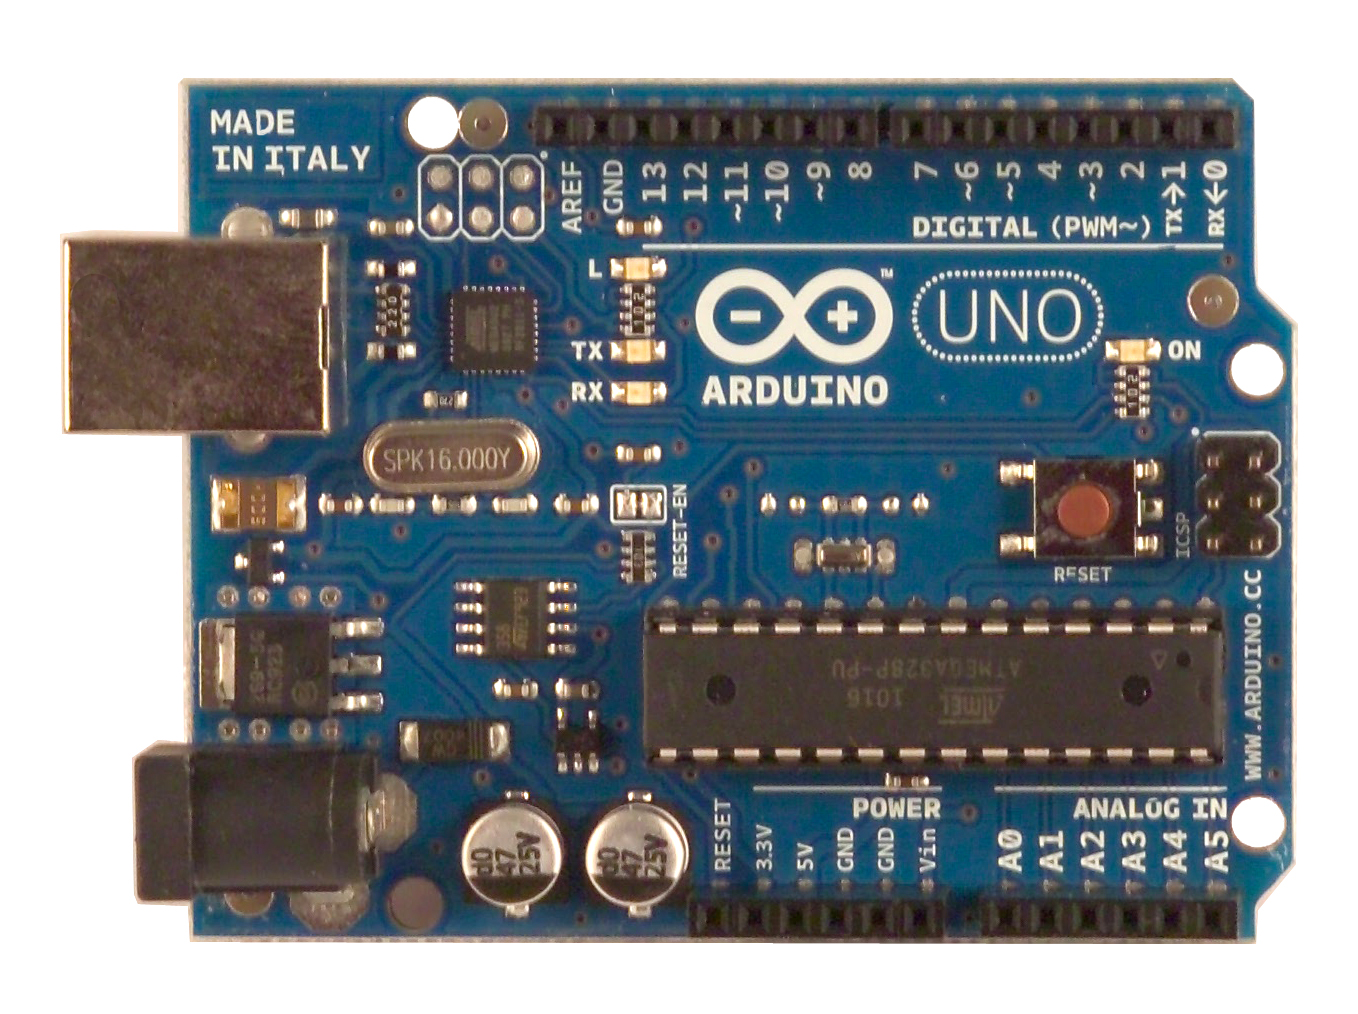
\includegraphics[width=120mm]{Media/www-arduino-cc_ArduinoUnoFront.jpeg}
  \caption{Arduino Uno}
  \label{ArduinoUnoFront}
\end{figure}



\begin{figure}[htbp]
  \centering
  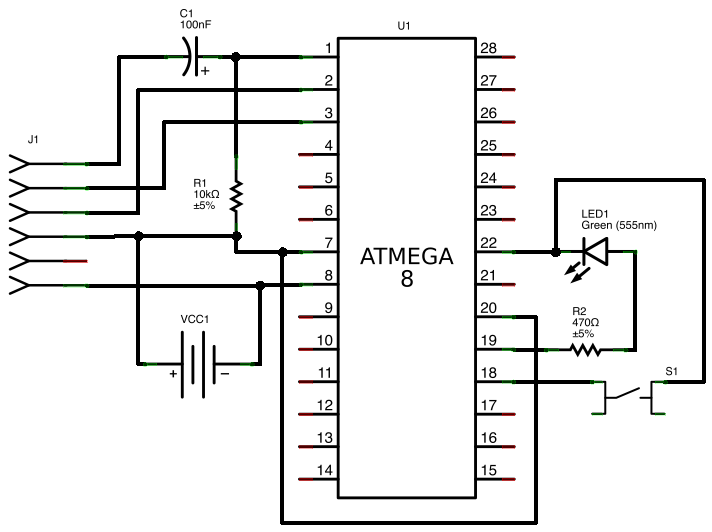
\includegraphics[width=120mm]{LED/S000_LED-Basic-Circuit_schema.png}
  \caption{Basic Schema}
  \label{atmega8-basic-schema}
\end{figure}

If not, you may build a circuit like in figure \ref{atmega8-basic-schema} on page \pageref{atmega8-basic-schema}. The breadboard layout is shown in file \texttt{LED/S000\_LED-Basic-Circuit.fz} in Fritzing file format.

As you may find out, we are focused on Free and Open Source Software. All published program code here is Free Software, the book itself and all used attachments are as free as we allowed to make them.

Also we will prevent usage of non free 'things' as hard as we can. We will not force anyone to use non free products to follow our ways. On of our main goals is an intellectual contribution to the world of Free Thinking, Libre Software and cooperative work.


!en \section{Let there be light!}
!de \section{Es werde Licht!}

!en The first sample in this chapter is the smallest program I can think of which does something.

!de Das erste Beispiel in diesem Kapitel ist das kleinste Programm, das ich mir vorstellen kann, das tatsächlich auch etwas sichtbares tut.



!en This program will switch on the LED on your Arduino pin 13.

!de Es schaltet die LED am Arduinoanschluss 13 ein.



!en Programming in Assembler means you're in control. But as you know, power requires knowledge and responsibility. If you're entering the world of assembly programming, you have absolute power if you wish to or not. Consequently you need knowledge to become responsible.

!de In Assembler Programmieren heisst, Du hast die Macht! Aber wie wir wissen, erfordert Macht Wissen und Verantwortungsbewusstsein. Jemand der Micro Controller in Assembler programmiert, hat die absolute Macht, ob er es will oder nicht! Demzufolge ist ein Mindestmass an Fachwissen erforderlich um verantwortlich zu handeln.



!en At first you need to know what 'Arduino pin 13' really means. As consequence of the Arduino design it is not pin 13 on your \at. Knowing this is yet the half way thru. Knowing the pin is a step you need to know if are working with a plain chip. What you need to know is the micro controllers internal addressing for Arduino pin 13. To find out, look at \url{http://www.arduino.cc/hu/Hacking/PinMapping}.

!de Als erstes musste Du wissen, was Anschluss 13 am Arduino in Wirklichkeit heisst. Infolge des Arduinodesigns ist Anschluss 13 am Arduino nicht Pin 13 am \at. Das zu wissen ist erst die halbe Miete. Das tatsächliche Pin am \at zu kennen ist erforderlich um mit dem blanken Chip zu arbeiten. Was Du ausserdem wissen musst ist, wie dieser Anschluss im Micro Controller adressiert werden muss. Um das alles heraus zu finden gibt es ein sehr schönes Schaubild: \url{http://www.arduino.cc/hu/Hacking/PinMapping}


\begin{figure}[htbp]
  \centering
  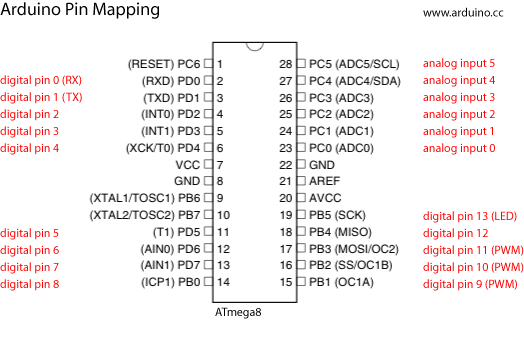
\includegraphics[width=120mm]{Media/www-arduino-cc_Arduino-To-Atmega8-Pins.png}
!en   \caption{Arduino to \at  pins}
!de   \caption{Arduino zu \at  Anschlusszuordnung}
  \label{arduino-to-atmega-pins}
\end{figure}

!en After we know everything we need to know to be responsible, we generate our 8byte program that will set our 'LED 13' under power.

!de Nachdem wir zunächst vermutlich genug wissen um verantwortungsvoll zu handeln, programmieren wir unser 8 Byte grosses Programm, dass 'Adruino LED 13' erleuchtet.


\begin{lstlisting}
; LED/S000_let-there-be-light.asm

.DEVICE atmega8

.org 0x0000
            rjmp    start 

start:
            sbi     DDRB,         5
            sbi     PORTB,        5
            
main:
            rjmp    main
\end{lstlisting}

!en As simple as the program is, I believe there is some need for explanation.

!de So einfach dieses Programm auch ist, es gibt doch ein paar Kleinigkeiten zu beleuchten.



!en At first we have to declare the type of micro controller we are intended to use with the program. This is necessary because different micro controllers do have different assignments in their inner structure and need different addressing for their components. The assembler need to know which values to assign for which elements. In our example the assembler needs to know who to address DDRB and PORTB. DDRB and PORTB are place holders or 'logical names' for numerical values. Declaring the micro controller assigned specific values to all such logical names. We do this by:

!de Zunächst müssen wir angeben, welchen konkreten Micro Controller wir verwenden. Das ist erforderlich weil die verschiedenen Modelle verschiedene Adressen für ihre Elemente aufweisen. Dem Assembler wird auf diese Weise mitgeteilt, welche Werte er für welche Elemente verwenden muss. In unserem Beispiel für DDRB und PORTB. DDRB und PORTB sind Platzhalte oder auch 'logische Namen' für Zahlen. Welche Zahlen verwendet werden, entscheidet die Microcontrollerangabe. Das geschieht durch:

\begin{lstlisting}
.DEVICE atmega8
\end{lstlisting}



!en Next we need to declare where our world will begin. Funny thing is, we will never really know! So we are forced to use symbols to deal with this necessity. As indicated below, different micro controllers will have different inner values. But not only this, to be honest, where our program lives is due to additional effects a most uncertain thing. We come to this later in the book.

!de Als nächstes müssen wir den Anfang der Welt benennen. Der Witz hierbei ist, dass wir die volle Wahrheit nie wirklich erfahren! Wir verwenden Symbole um mit dieser Anforderung umzugehen. Wie bereits beschrieben, haben verschiedene Micro Controller verschiedene innere Werte. Aber nicht nur das. Wo exakt sich unser Programm am Ende tatsächlich befinden wird ist eine kaum beantwortbare Frage. Später werden wir nochmals darauf zurück kommen.


!en As we are forced to use symbols, we have to do so. We will set a symbol to our programs starting point later and this symbol will be named 'start' in out code. Whatever starts our program it must be informed where to goto to do so:

!de Da wir also zur Verwendung von Symbolen gezwungen sind, werden wir dementsprechend handeln. Wir werden mit einem Symbol den Startpunkt unseres Programms markieren. Dieses Symbol werden wir 'start' nennen. Was immer auch unser Programm starten wird, es muss diesen ominösen Startpunkt kennen:

\begin{lstlisting}
.org 0x0000
            rjmp     start 
\end{lstlisting}



!en With '\texttt{.org}' (don't forget the leading dot!) we build a sequence of commands positioned at the addressed position. This sequence, some times named a table, is a list of actions to do for different requests. At the moment he only request we have is to start our program and fortunately the entry for this request is expected as the first in our table.

!de Mit '\texttt{.org}' (bitte den Punkt am Anfang nicht vergessen) eröffnen wir eine Sequenz von Befehlen, die an der bezeichnete Position (hier 0x0000) beginnt. Diese Sequenz, die auch Tabelle genannt wird, ist eine Liste von Aktionen, die für bestimmte Anforderungen ausgeführt werden sollen. Für unser Programm besteht die einzige Anforderung darin, unser Programm zu starten. Und glücklicher Weise findet sich der Eintrag für diese Anforderung, also 'Starte das Programm', an der ersten Stelle diese Tabelle.



!en For those who really want to know: The addressing in this table is relative to wherever it is placed in real life! So it always starts with 0. Strictly speaking, at this point we already enter the realms of a dreamworld. We don't know what really happens! But sometimes we don't need to. To declare our first magic point, we only need to postulate:

!de Für die Neugierigen unter uns: Die Adressierung innerhalb dieser Tabelle, ist immer relativ zum Anfang der Tabelle. Die Tabelle befindet sich in Wirklichkeit kaum an der Position \texttt{0x0000}, aber darauf müssender keine Rücksicht nehmen. Genau genommen betreten wir hier bereits eine Art Traumwelt: Wir wissen nicht wirklich, was passiert! Aber in manchen Fällen, wie hier, müssen wir das nur sehr selten wissen. Um unseren ersten 'Magischen Weltpunkt' zu bestimmen, formulieren wir lediglich:

\begin{lstlisting}
start:
\end{lstlisting}



!en '\texttt{start:}' is a label and represent the final address for the first memory position used afterwards. In our case the address of the first command in our program.

!de '\texttt{start:}' ist eine Marke, ein Label. In unserem Fall ist es eine Sprungmarke. Sie repräsentiert die Adresse der ersten Speicherstelle nach ihrem Erscheinen. In unserem Fall die Adresse des ersten Befehls unseres Programms.



!en The next label is already behind all things we need to do in our program. It is the starting point of an unconditional infinite loop. This sequence is necessary because the processor (CPU) of our micro controller (MC) is running as long as it has power. We can't stop it, so we have to lead it into a controlled way of doing 'nothing' because we don't wish our MC to do anything after it did all things we expected it to do.

!de Die nächste Sprungarke befindet sich bereits hinter dem eigentlichen Ende unseres Programms. Sie ist der Beginn einer unbedingten unendlichen Schleife. Diese Schleife ist erforderlich, weil der Prozessor (CPU) unseres Micro Controllers (MC) operiert, solange er Strom hat. Diese Aussage stimmt nicht, in Wirklichkeit kann man nicht nur die CPU anhalten. Das Anhalten der CPU ist aber bereits ein recht komplizierter Vorgang. Wichtig, aber kompliziert. Darum tue ich hier so als wäre es nicht möglich. Da wir die CPU also (momentan) nicht stoppen können, müssen wir ihr etwas zu tun geben was das Ergebnis unseres Programms nicht beeinträchtigt.



!en Between '\texttt{start:}' and '\texttt{main:}' is our program. I call this the 'first form of a standard program'. A program which runs ones after the system awakes. Such program may be of limited use, but not completely useless. The schema of this 'first form' is the basic schema of all derived forms. The program 

!de Zwischen '\texttt{start:}' und '\texttt{main:}' befindet sich momentan unser eigentliches Programm. Ich nenne das ein Programm der 'Ersten Form'. Ein solches Programm mag nur begrenzten Nutzen haben, aber es ist ganz sicher nicht völlig sinnlos. Diese 'Erste Form' ist die Basis aller erweiterten Programmformen. Ein solches Programm

\begin{itemize}
!en   \item  starts
!de   \item  startet
!en   \item  does something
!de   \item  tut etwas
!en   \item  loops forever, doing nothing
!de   \item  tritt in eine Endlosschleife, tut nichts mehr
\end{itemize}



!en If the program does something inside the 'infinite loop' then this may be called the 'second form of a standard program'. A third form should be expected to pop into existence later on. But anyway, our current program of the first form is specifically designed to show some important rules for good MC programming.

!de Sofern das Programm im inneren der Endlosschleife etwas tut, nenne ich das die 'Zweite Form' eines Programms. Eine 'Dritte Form' darf für später erwartet werden. Sei es wie es sei, unser aktuelles Programm wurde speziell entworfen um einige wichtige Regeln guter MC Programmierung zu demonstrieren.


!en The two commands which full fill our programs mission will do two things:

!de Die beiden Befehle, die die Aufgabe unseres Programms erfüllen tun das folgende:

\begin{itemize}
!en   \item  declare pin 5 at PORTB as output pin
!de   \item  Bit 5 an PORTB als Ausgabepin festlegen
!en   \item  set pin 5 at PORTB under power to enlighten our LED
!de   \item  Bit 5 an PORTB einschalten um die LED zu erleuchten
\end{itemize}

\begin{lstlisting}
            sbi     DDRB,         5
            sbi     PORTB,        5
\end{lstlisting}

!en Finally the never ending loop:

!de Am Ende die nicht enden wollende Schleife:

\begin{lstlisting}
main:
            rjmp    main
\end{lstlisting}

!en This is all the program does and there is nothing more about it. You will discover, that this program demonstrates prudence and thrift. 

!de Das ist alles was das Programm tut. Allerdings wirst Du feststellen, dass dieses Programm bedacht und sparsam operiert.


!en A PORT of an 8bit MC controls eight bit unsing eight pins on the outside. In our \at{} each one of these pins can be used to:

!de Ein PORT eines 8bit Micro Controllers verwaltet 8 Bits um 8 Beine in der Aussenwelt zu steuern. An unserem \at{} kann jedes dieser Beine verwendet werden um eine der folgenden Funktionen zu erfüllen:

\begin{itemize}
!en   \item Put a signal to his pin
!de   \item Ein Signal ausgeben
!en   \item Read a signal from its pin which may be +5V or GND as 1 or 0
!de   \item Ein Signal lesen, dass +5V oder GND ist als Repräsentation für 1 or 0
!en   \item Read a signal from its pin which may be 'not GND' or GND as 1 or 0
!de   \item Ein Signal lesen, dass 'nicht GND' oder GND ist als Repräsentation für 1 or 0
\end{itemize}

!en Each pin as can be controlled to do one of these things freely, independent of all the other pins on the same port.

!de Jedes Bein kann unabhängig von jedem anderen Bein konfiguriert werden um eine dieser Operationen auszuführen. Alles am gleichen Port!



!en On some pins are additional features possible like

!de An einigen Beinen sind weitere Funktionen möglich wie

\begin{itemize}
!en   \item power saving modes (the pin becomes deaf)
!de   \item Energiesparmodus (das Bein wird abgeschaltet)
!en   \item PWM modes
!de   \item Pulsbreitenpodulierter Signalgenerator
!en   \item analog to digital converting
!de   \item Analog-Digital-Wandlung
!en   \item interrupts
!de   \item Interruptempfang
\end{itemize}

!en In our program we use the command \texttt{sbi} to set bit 5 instead of the alternative command \texttt{out} with parameter \texttt{1 << 5} which would do the same but not really the same. We wish to manipulate bit 5 only! \texttt{out 1 << 5} would not only send \texttt{1} to bit 5 but also \texttt{0} to all other pins.

!de In unserem Programm verwenden wir den Befehl \texttt{sbi} um das Bit 5 anzusteuern anstatt den Befehl \texttt{out} mit dem Parameter \texttt{1 << 5} zu verwenden, was auf den ersten Blick zum gleichen Ergebnis führen würde. Wir wollen aber einzig bit 5 ansteuern! \texttt{out 1 << 5} würde dummer Weise aber nicht nur Bit 5 auf \texttt{1} setzen, sondern gleichzeitig alle anderen Bits, ihrer 7 Stück, auf \texttt{0}!


!en Even if we - at the moment - know that all other pins are unused, we face to situations:

!de Auch wenn wir - für den Augenblick - wissen, dass alle anderen Bits nicht benutzt sind, werden wir bald mit den eher typischen Situationen konfrontiert:

\begin{enumerate}
!en   \item We will become less and less sure about the usage of bits we don't use in a particular situation. Especially if we are developing a library.
!de   \item Wir werden zunehmen unsicher werden, welche Bits tatsächlich benutzt werden, während wir etwas bestimmtes programmieren. Auch und besonders wenn es sich um Bibliotheken handelt. Dann sowieso nicht!
!en   \item We don't know what happens if we send \texttt{0}'s to pins we don't know.
!de   \item Wir wissen nicht was passiert wenn wir \texttt{0} an Bits senden, die wir momentan gar nicht betrachten.
\end{enumerate}



!en \emph{One major concept of good programming is, to do as less as any possible.}

!de \emph{Ein wichtiges Konzept guten Programmierstils ist, so wenig wir irgend möglich zu tun.}



!en If there is nothing to be done, don't do it! Especially in micro controllers where action means energy loss. So if we need to manipulate a bit, we should not manipulate others bits except we have a good reason to do so. Currently we have not.

!de Wenn nichts zu tun ist, dann tu's nicht! Das gilt besonders bei Micro Controllern, wo jede Aktion Energieverbrauch bedeutet. Wenn wir also ein Bit ansteuern wollen, sollten wir genau ein Bit ansteuern und nicht mehr, ausser wir haben gut Gründe, diese Regel nicht zu beachten. Momentan haben wir die nicht.



!en We don't want to wake up pins if they could sleep in peace. Because possibly, these otherwise unused pins will eat up our energy.

!de Wir wollen nicht Beine Aufwecken, wenn sie auch in Ruhe schlafen könnten. Denn möglicher Weise würden diese Anschlüsse alle zur Verfügung stehende Energie verheizen, im Sinn von heizen!

\section{Get me on - Get me off}

At first the enhanced schema

\begin{figure}[htbp]
  \centering
  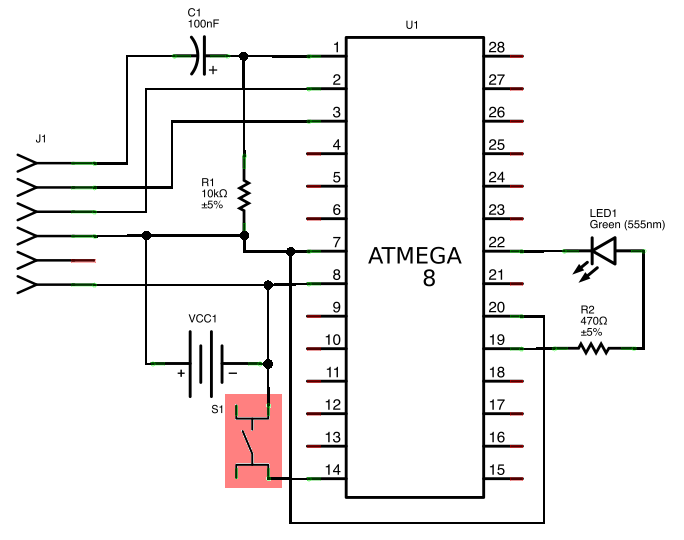
\includegraphics[width=120mm]{LED/S002_get-me-on-get-me-off_Circuit_schema.png}
  \caption{Basic Schema}
  \label{atmega8-get-me-on-get-me-off-schema}
\end{figure}


Second the code


\begin{lstlisting}
; LED/S002_get-me-on-get-me-off.asm

.DEVICE atmega8

.org 0x0000
           rjmp     start

start:
            sbi     DDRB,         5
            cbi     DDRB,         0
            sbi     PORTB,        0

main:
            sbic    PINB,         0
            rjmp    led_on
            cbi     PORTB,        5
            rjmp    led_ok
led_on:
            sbi     PORTB,        5
led_ok:
            rjmp    main
\end{lstlisting}

As you may have guessed, this code represents the 'second form of a standard program'. It does something before the loop - ones - but also does something in the main loop. This program is really busy as we will see in the next program.

The first difference to the former program is, that we use an additional pin/bit. This time for input. To set this pin, bit 0 on port B at pin 14 of the micro controller, to input mode, we send a '0' to its data direction register (DDR). Further we send a '1' to this bit 0 of the port as if we would set the port to output +5V. But this bit is in 'output mode'. In this case, sending '1' to the bit at the port means: 'Switch on the internal pull-up resistor!'

After this, the signal read from this bit is 'ON' or '1'. To interact with the micro controller and change the signal to OFF, we need to pull-down the pin to GND.

If we do so, our program switches the light off as long as we ground bit 0, which does not make real impressive application to boast around with. For us it is great anyway because we understand what happens.

If you follow the programs flow:

\begin{enumerate}
  \item Initialise system and devices
  \item Read bit 0
  \item Set bit 5 accordingly
  \item Start with (2)
\end{enumerate}

You may ask why we permanently output a signal that nearly never changes. Assuming our program reads the input bit one million times per second, a human will not be able to put any business to this program by flipping the switch on and off. If you pick on your signal line as fast as you can then in the eye of your program the signal nearly never changes.

Is there room for optimisation? We believe not.

Are there alternatives? Yes there are!

We could save the output status, compare the status from the input bit with the stored status the light was set to and only change the output signal if the input signal has changed.

This sounds easy, but it is not! It is not only not easy, it is dangerous, costly and complicated. And it is of no use, because you do a lot of commands without any effect.

The concept is dangerous because you may be out of synchronisation with your light. In this case you light may react inverse to your intension or does not react at all.

It is costly not only because the program would be much larger but you need to eat up one CPU register and we only have 32 of them at all.

And it is complicated because you have to synchronise two entities (the light and the status register) to generate one effect. Which is a major risk and drawback.

Because of this, we might be right in our assumption that the developers of our \at micro controller created the chip in such a way that nothing happens if we switch on a bit that is ON already.

Another alternative may be to 'stop' the program as long as it waits for the input signal to change. This may be possible, but it lies far behind our current knowledge.

There is no command that makes the micro controller wait for an input signal. But there are ways to reach a similar effect.

Which means, for now we are out of options and have to stay with the solution as presented in this section. But we will come to status management later.
\section{Stable Decisions}

Next step we need to do something more useful. And we reach the 'second form of a standard program', which means: A program that does something in its infinite loop.

This program stores one of two states ;-) and sets the light on or off, keeping it according to the stored status. This explanation is slightly wrong. I try it again.

This program recognises an input signal consisting of two phases. A complete input signal consist of a LOW phase starting from a HIGH phase followed by the next HIGH phase. The signal ends with entering the HIGH phase. We are interested only in change, as we always should.

If the Input signal changes from HIGH to LOW, our program changes the light from its current status to the other status. If the light was ON it will be set to OFF and vice versa. The status is only changed as reaction of changing the Input from HIGH to LOW because 'no action' at the Input device leads to HIGH status in the input register as the result of using an internal pull-up resistor who does what he is called - he pulls the input signal up to HIGH.

The electrical signal we are waiting for with our micro controller on our input pin is: Pulling the status down to LOW (GND). We may phrase:

\begin{center}
The \emph{Signal} we are waiting for it the \emph{Change} form HIGH to LOW.
\end{center}
 

So for the first time we have to be aware of a dynamic process. If the Change is the Signal, then we have to recognise if the status is change. If a status appears after the opposite status was recognised before - in the past - which is no more present (!) we have to deal with 'historical' status management and so for the first time with remembering a status from one processing cycle to the next.

Finally this here is the Code to do it:

\begin{lstlisting}
; LED/S004_stable-decisions.asm

.DEVICE atmega8

.org 0x0000
            rjmp    start

start:
            sbi     DDRB,         5
            cbi     DDRB,         4
            sbi     PORTB,        4

            ldi     r16,          1

main:
            sbic    PINB,         4
            rjmp    led_keep
            tst     r16
            breq    led_ok
            clr     r16
            sbis    PINB,         5
            rjmp    led_on
            cbi     PORTB,        5
            rjmp    led_ok
led_on:
            sbi     PORTB,        5
            rjmp    led_ok
led_keep:
            ldi     r16,          1
led_ok:
            rjmp    main
\end{lstlisting}


As you can see, this Code is not easy to understand. To do better, we add symbolic names to the soup. The basics are easy:

\begin{itemize}
  \item \texttt{.equ} means: 'a name for a number'
  \item \texttt{.def} means: 'a name for an entity'
\end{itemize}

So for example \texttt{DDRB} alread is a number. This number is defined in an include file chosen by you device selection. But in our case, whatever number is hidden behind the name DDRB it will be our Input/Output control port. So die name it \texttt{ctl} as prefix for 'control' and \texttt{IO} as name for Input\&Output.

In another example \texttt{bit} stands for 'bit number' and \texttt{Input} for 'Input bit' which makes \texttt{bitInput}, the bit where we red the input state.

You may define you own naming convention which should hold throughout your project.

\begin{lstlisting}
; LED/S005_stable-decisions+symbols.asm

.DEVICE atmega8

.equ ctlIO     = DDRB    ; DDRB  is our I/O control register
.equ prtIO     = PORTB   ; PORTB is our I/O output port register
.equ pinIO     = PINB    ; PINB  is our I/O input pin register

.equ bitOutput = 5       ; pin 5 is our output bit
.equ bitInput  = 4       ; pin 4 is our input bit

.equ FALSE     = 0       ; 0 will be FALSE or OFF
.equ TRUE      = 1       ; 1 will be TRUE  or ON

.def bStatus   = r16     ; the last state will be stored in 'r16'
\end{lstlisting}

As you may not have expected, this makes the soup - or code - somehow better readable and so much easier to understand. Now it looks more like a higher language:

\begin{lstlisting}
.org 0x0000
            rjmp    start

start:
            sbi     ctlIO,        bitOutput
            cbi     ctlIO,        bitInput
            sbi     prtIO,        bitInput

            ldi     bStatus,      HIGH

main:
            sbic    pinIO,        bitInput
            rjmp    led_keep
            tst     bStatus
            breq    led_ok
            clr     bStatus
            sbis    pinIO,        bitOutput
            rjmp    led_on
            cbi     prtIO,        bitOutput
            rjmp    led_ok
led_on:
            sbi     prtIO,        bitOutput
            rjmp    led_ok
led_keep:
            ldi     bStatus,      HIGH
led_ok:
            rjmp    main
\end{lstlisting}

Even if it's a better reading, it seems no really to be easy to follow the program flow. So at first, we should introduce a program flow chart. And for good measure two of the. We need two of them to demonstrate a major point in assembler programming.

We have to take watch about WHAT we wish to do, but equally too about HOW we are going to do it.

\subsection{WHAT to do}

\begin{enumerate}
  \item Initialise system and devices
  \item Wait for the change "input pin was HIGH and became LOW"
  \item Invert LED status
  \item Restart at (2)
\end{enumerate}


\subsection{HOW to do it}

To get an impression on how to it, at first, we take a look at a flow diagram. This diagram shows the program flow outside the 'invert LED status' part. Changing the LED status currently is out of our focus. It is the very thing we try to deal with, but it is the more easy part of the solution.

\begin{figure}[htbp]
  \centering
  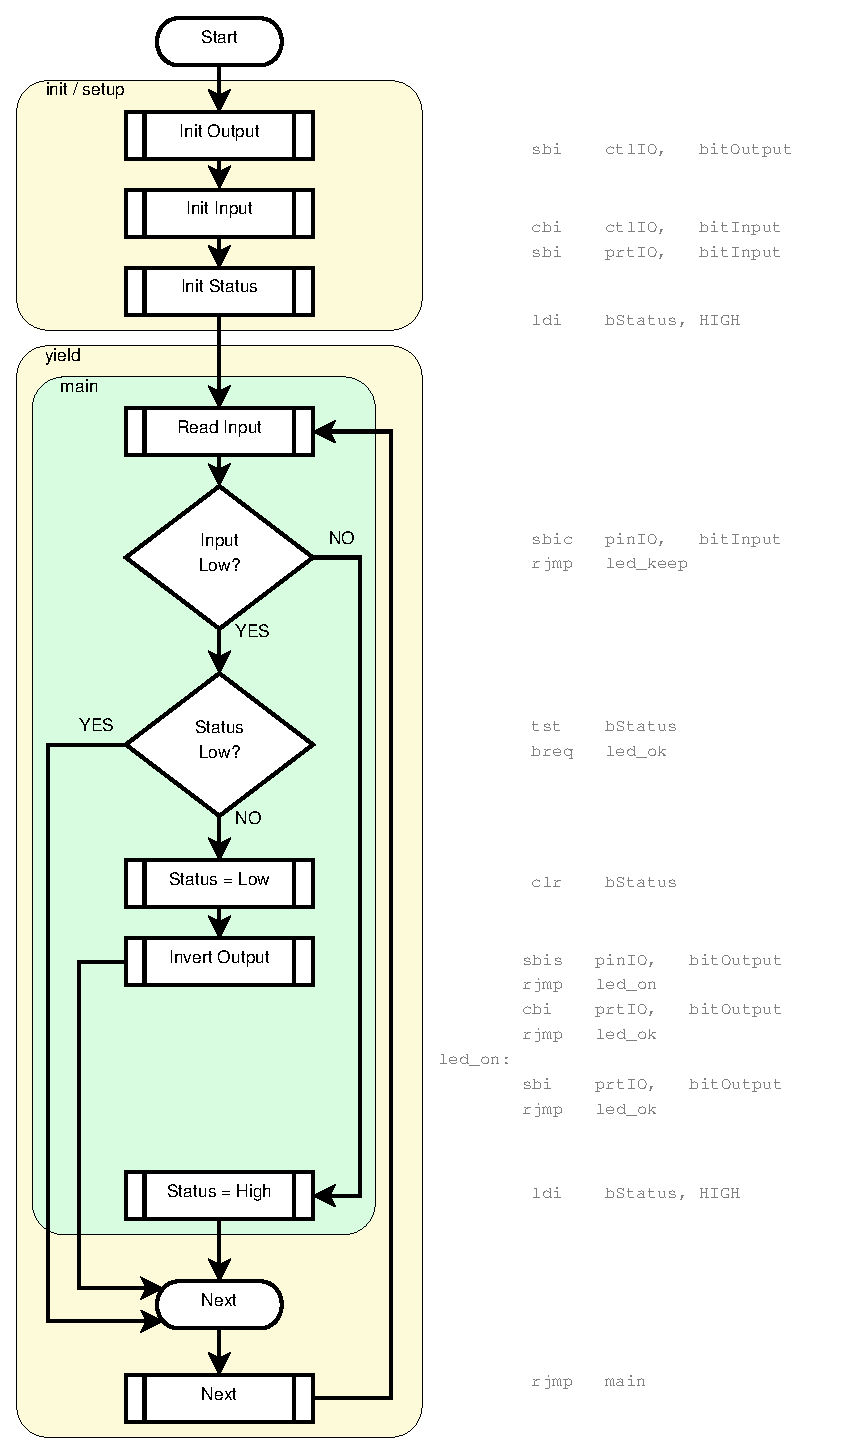
\includegraphics[height=210mm]{LED/S005_stable-decisions+symbols.eps}
  \caption{Stable Decisions Flow Diagram}
  \label{S005FlowDiagam}
\end{figure}

As you may found out until now, dealing with the 'human device interface' is the most complicated thing in informatics. It starts by the unbearable slowness of humans and does not end with humans expectations against machines.

At the moment out project restricts the 'human device problem' the unbearable slowness of humans.

A living entity presses a button and our device has to react. Our device may ask the input pin about 1.000.000 times per second. A human for example may to a short pressing of the button in about 0.2 seconds. Which means, our System reads the state 'button pressed' about 500.000 times during our humans action. But what the human expects is:

"Change the LED status ones as I press (in my view) the button ones!"

A second problem we will not deal with in this phase of our development is, that electric switches may flicker during status change.

So we simply have to ensure, that changing the LEDs status only happens ones per button press action. There are only two moments in all this endless button down phase where it is suitable to really change the LEDs status. At the beginning, as the signal changes from HIGH to LOW or at the end, where the signal changes from LOW to HIGH again.

To give the human who uses our device immediate feedback about success or failure of his action, we decide to use the first phase to do all the action. So we have a simple mission: If the signal is LOW now and was HIGH the last time we looked, we change the LEDs state. This satisfies also the endless LOW state of the input signal and the change from LOW to HIGH where we have to do nothing. Not even accidentally! This way, the human feels his request immediately answered, even if he is unable to comprehend how immediately it real is answered.


\subsection{Finding the right moment}

To find the moment the signal has gone to ground, we have to be aware of the status of the signal from the previous query cycle. Which is easy but expensive. We simply use a register to store the previous input status.

So we simply have to check if the last seen status was HIGH as log as the current status is LOW. The status accumulator register follows the status of the input signal after being used to query the change event.

If the one moment we are waiting for passes, we invert the LED status. That's all

\subsection{And some modesty}

In respect of things to come, we have to be modest in our style. The 'endless loop' which keeps the micro controller running and waiting without going wild, will be used for some important things:

\begin{itemize}
  \item It mostly contains the main program
  \item It possibly consist of multiple parts to do
  \item It consist of an unknown amount of program parts
\end{itemize}

So we have to ensure, to don't make any shortcut back to the 'main' label. As there can only be one Highlander, there can only be one jump back to 'main'. This jump resides at the very end of the main sequence.

In our flow diagram one part has to reach the next part regardless of how the program flow is flowing. The rounded rectangle 'next' represents the central point behind our (currently) one part. This is the position where the next program part will follow in the same manner.


\section{Light Shift}

Next we will start with showing off. A little bitt at least. We will put three lights in a row and lighten one of them up each time we press the button.

It would be much easier to do this with 8 lights, but here we are. We will keep the existing circuit as untouched as possible and, not at last, we are constantly on he search for a challenge.

So here is the code:

\begin{lstlisting}
; LED/S010_light-shift.asm

.DEVICE atmega8


.equ ctlIO         = DDRB
.equ prtIO         = PORTB
.equ pinIO         = PINB

.equ bitSignal     = 5
.equ bitInput      = 4
.equ bitLightStart = 3

.equ mskLightShift = 0x0E

.equ LOW           = 0
.equ HIGH          = 1

.def bStatus       = r16
.def bTemp         = r17
.def bData         = r18


.org 0x0000
            rjmp    start


start:
            ldi     bTemp,        mskLightShift | 1 << bitSignal
            out     ctlIO,        bTemp
            ldi     bTemp,        1 << bitInput | 1 << bitSignal
            out     prtIO,        bTemp

            ldi     bStatus,      HIGH

main:
            sbic    pinIO,        bitInput
            rjmp    led_keep
            tst     bStatus
            breq    led_ok
            clr     bStatus

            in      bData,        pinIO
            mov     bTemp,        bData
            andi    bData,        0xFF - mskLightShift
            ori     bData,        1 << bitInput

            andi    bTemp,        mskLightShift
            lsr     bTemp
            andi    bTemp,        mskLightShift
            brne    shift_ok
            ldi     bTemp,        1 << bitLightStart
shift_ok:
            or      bData,        bTemp
            out     prtIO,        bData

            rjmp    led_ok
led_keep:
            ldi     bStatus,      HIGH
led_ok:
            rjmp    main
\end{lstlisting}

As you can see, we have some changes to the former code. This is, in the hole, because we will deal with four instead of one lights. One light (the one we toggled last time) will serve as signal light, lighting up after out micro controller has finished booting. The other will used to shift the light. In our case, this means, we start off with one light ON and each time we press our button the next light lights up whilst the former active light shuts off.

Our code reflects this at the first look with more constants and more named registers. Already we are using 10\% of all registers present and 20\% of all registers usable for generic purpose. This is bad news! Hopefully our resource consumption will not grow with constant speed.

Names for values (not resources) we need besides the ones from the former sample are

\begin{lstlisting}
.equ bitLightStart = 3     ; as in  0b00001000

.equ mskLightShift = 0x0E  ; builds 0b00001110
\end{lstlisting}

\texttt{bitLightStart} is the number of the pin on the output port where the first LED of our LED chain resides. The other LEDs are expected to use the two lower pins (2 and 1). Pin B0 on the \at can be found on the other side of the chips, so for our physical breadboard circuit it's a bit too complicated to use it.

Please remember, such decisions are no fun. In reality you may sometimes be driven to compensate in software for simplification of hardware as PCB layout, different chips and so on. So we accept this situation as example of what may happen in real life.

\texttt{mskLightShift} is a bit mask containing bits ate all pins of the output port where our light chain is connected to. We need such a bit mask because we need to shift the 'LED ON' bit around but won't shift any other bits found in the port data.

Named registers (resources) we need in addition are:
 
\begin{lstlisting}
.def bTemp         = r17
.def bData         = r18
\end{lstlisting}

\texttt{bTemp} will be used to shift our 'lED ON' bit around but \texttt{bData} has to give us the 'big picture' about our ports status. First before, second after shifting the 'LED ON' bit.

We start, as usual, by initialising the micro controller where it needs to be initialised. This time, we need to set all pins on our port the same time because the alternative is (for the moment) not acceptable. So we build a bit mask to send it to our IO ports data direction register (DDR):

\texttt{mskLightShift} combined with \texttt{1 << bitSignal} makes \texttt{0b00101110}. Sending this byte to DDRx will set pins 1, 2, 3, 5 to output and all other pins to input mode.

\begin{lstlisting}
start:
            ldi     bTemp,        mskLightShift | 1 << bitSignal
            out     ctlIO,        bTemp
            ldi     bTemp,        1 << bitInput | 1 << bitSignal
            out     prtIO,        bTemp
\end{lstlisting}

Then we need to do three things by sending a byte to PORTx:

\begin{itemize}
  \item Switch ON LED on pin 5 (\texttt{bitSignal})
  \item Set pin 4, our input pin, to 'pulled up' (\texttt{bitInput})
  \item Set all other pins to off/offline
\end{itemize}

All this is done by mixing all active bits together and sending the mix \texttt{(0b00110000)} to the port. After doing so the signal LED is on, the light chain is off. Until \texttt{clr bStatus} nothings more has changed. Also the rest with and after label \texttt{led\_keep} is kept the same.

The changed part is this:

\begin{lstlisting}
            in      bData,        pinIO
            mov     bTemp,        bData
            andi    bData,        0xFF - mskLightShift
            ori     bData,        1 << bitInput

            andi    bTemp,        mskLightShift
            lsr     bTemp
            andi    bTemp,        mskLightShift
            brne    shift_ok
            ldi     bTemp,        1 << bitLightStart
shift_ok:
            or      bData,        bTemp
            out     prtIO,        bData
\end{lstlisting}

All magic resides in these lines. It's not too much, so we simply explain it sequentially.

We need to get the ports state and unfortunately we have to understand more about this than is good for the program. We have to send back the whole data byte, modified only in the part where the LED chain state changed. BUT (!) we also need to ensure, our input pin keeps his pull up resistor active. Otherwise we loos our connection to the outer world!

Next we need to split the read byte/data in two parts. The one containing constant data and the other one containing the bits to be shifted.

Phase one therefore copies \texttt{bData} to \texttt{bTemp}, then masks out all bits dealer with in the bit shifting process and finally adding/regenerating the 'pull up' bit for port \texttt{bitInput}.

Phase two masks out all bits not related to the bis shifting operation, shifts the remaining bit and masks the result again with the same mask. If this operation leads to a result of ZERO/EQ/NULL, then we have shifted out our bit and need to insert a new bit at the start position inside the byte \texttt{bitLightStart}.

Phase three then combines our static bits with our manipulated one and put all together to our combined input/output port.



\chapter{Time}

\section{Instable Elements}

The longest time we tried to avoid the simplest demo in most Arduino beginners sets. The blinking light demo! Some of our readers may have ask themselves where the problem should be. Now is the moment to explain.

We do not want to make a fuss with code we would have to be ashamed of but couldn't bring us to start with timers and interrupts before introducing the most basic principles of programming. Please remember, using assembler language brings us in a position of power which forces us into reliability.

There is no way a reliable programmer would use 4.000.000 NOPs ('no operation' operations) twice to let a light blink ones per second. Also, we hope, no one reading until this point would keep it as responsible to enter a loop, busying our poor micro controller to wait half a second by wasting four million CPU cycles.

So we had to experiment enough to enter the reign of timers and interrupts. Staying our ground not demonstrating bad code, keeping the book pure, we don't show only a part of a single bad example in code. You may remember it in your dreams!

To cut a long story short. Here its the code:

\begin{lstlisting}
; LED/S020_instable-elements.asm

.DEVICE atmega8

.org 0x0000
            rjmp    start 

start:
            ...            
main:
            rjmp    main
\end{lstlisting}



\part{External devices}

\chapter{Shift Registers}

\section{SRAM to Shift Register}

Sending SRAM content/data to shift registers has some applications. Some of them are

\begin{itemize}
  \item {Light chains}
  \item {Raster displays}
\end{itemize}

It is an important way to communicate with the technical environment in certain situations. Most importantly if you have more bit to output as pins on your micro controller.

\end{document}
